El algoritmo de Kruskal es un algoritmo de la teoría de grafos para encontrar un árbol recubridor mínimo en un grafo conexo y ponderado. Es decir, busca un subconjunto de aristas que, formando un árbol, incluyen todos los vértices y donde el valor total de todas las aristas del árbol es el mínimo. Si el grafo no es conexo, entonces busca un bosque expandido mínimo (un árbol expandido mínimo para cada componente conexa). El algoritmo de Kruskal es un ejemplo de algoritmo voraz. Funciona de la siguiente manera

\begin{itemize}
	\item[-] Se crea un bosque B (un conjunto de árboles), donde cada vértice del grafo es un árbol separado.
	\item[-] Se crea un conjunto C que contenga a todas las aristas del grafo.
	\item[-] Mientras C es no vacío.
	\begin{itemize}
		\item[*] Eliminar una arista de peso mínimo de C.
		\item[*] Si esa arista conecta dos árboles diferentes se añade al bosque, combinando los dos árboles en un solo árbol.
		\item[*] En caso contrario, se desecha la arista
	\end{itemize}
\end{itemize}
Al acabar el algoritmo, el bosque tiene un solo componente, el cual forma un árbol de expansión mínimo del grafo.

Dada una lista de las aristas del grafo, el primer paso del algoritmo de Kruskal es ordenarlas por peso (usando un quicksort por ejemplo). Luego se van procesando las aristas en el orden de su peso, agregando aristas que no produzcan ciclos en el MST. El algoritmo de Kruskal es de O(A*log$_{ 2}$ A), donde A es el número de aristas del grafo.

El siguiente ejemplo ilustra el funcionamiento del algoritmo. La secuencia de ilustraciones va de izquierda a derecha y de arriba hacia abajo.

\begin{figure}[h]
	\centering 
	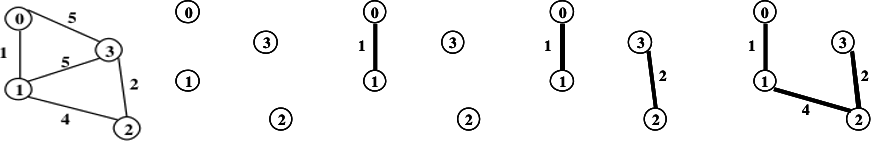
\includegraphics[scale=0.4]{img/kruskal}
	\caption{Ejecucción del algoritmo Kruskal.}
	\label{contexto:figura2}
\end{figure}

Este algoritmo fue publicado por primera vez en Proceedings of the American Mathematical Society, pp. 48–50 en 1956, y fue escrito por Joseph Kruskal. A continuación se muestra un seudocódigo del algoritmo.

\begin{lstlisting}
function Kruskal(G)
   Para cada v en V[G] hacer
      Nuevo conjunto C(v)\textleftarrow {v}.
   Nuevo heap Q que contiene todas las aristas de G, ordenando por su peso.
   Defino un arbol T ={ vacio }     
   // n es el numero total de vertices
   Mientras T tenga menos de n-1 vertices hacer
      (u,v) igual Q.sacarMin()
      // previene ciclos en T. agrega (u,v) si u y v estan diferentes componentes en el conjunto. 
      // Notese que C(u) devuelve la componente a la que pertenece u.
      if C(v) distinto C(u) then
         Agregar arista (v,u) a  T.
         Merge C(v) y C(u) en el conjunto
   Return arbol T
\end{lstlisting} 